% Very simple template for lab reports. Most common packages are already included.
\documentclass[a4paper, 11pt]{article}
\usepackage[utf8]{inputenc} % Change according your file encoding
\usepackage{graphicx}
\usepackage{url}
\usepackage{fourier}
\usepackage{listings}
\lstset{
  morekeywords={abort,abs,accept,access,all,and,array,at,begin,body,
      case,constant,declare,delay,delta,digits,do,else,elsif,end,entry,
      exception,exit,for,function,generic,goto,if,in,is,limited,loop,
      mod,new,not,null,of,or,others,out,package,pragma,private,
      procedure,raise,range,record,rem,renames,return,reverse,select,
      separate,subtype,task,terminate,then,type,use,when,while,with,
      xor,abstract,aliased,protected,requeue,tagged,until,public,static,void},
  sensitive=f,
  morecomment=[l]\#,
  morestring=[d]",
  showstringspaces=false,
  basicstyle=\small\ttfamily,
  keywordstyle=\bf\small,
  commentstyle=\itshape,
  stringstyle=\sf,
  extendedchars=true,
  columns=[c]fixed,
  numbers = left,
  numberstyle=\tiny,
  stepnumber=2,
  numbersep=5pt,
  framexleftmargin=5mm,
  language=R,
  frame=shadowbox
}

% CI-DESSOUS: conversion des caractères accentués UTF-8 
% en caractères TeX dans les listings...
\lstset{
  literate=%
  {À}{{\`A}}1 {Â}{{\^A}}1 {Ç}{{\c{C}}}1%
  {à}{{\`a}}1 {â}{{\^a}}1 {ç}{{\c{c}}}1%
  {É}{{\'E}}1 {È}{{\`E}}1 {Ê}{{\^E}}1 {Ë}{{\"E}}1% 
  {é}{{\'e}}1 {è}{{\`e}}1 {ê}{{\^e}}1 {ë}{{\"e}}1%
  {Ï}{{\"I}}1 {Î}{{\^I}}1 {Ô}{{\^O}}1%
  {ï}{{\"i}}1 {î}{{\^i}}1 {ô}{{\^o}}1%
  {Ù}{{\`U}}1 {Û}{{\^U}}1 {Ü}{{\"U}}1%
  {ù}{{\`u}}1 {û}{{\^u}}1 {ü}{{\"u}}1%
}
%opening
\title{Report 1: HTTP server}
\author{Simon Cathébras}
\date{\today{}}

\begin{document}

\maketitle

\section{Introduction}

During the preparation of this seminar, we did an implementation of an HTTP server in Erlang. This server was made following instructions provided in the subject.
During this preliminary study, we studied HTTP protocol, the use of a socket API, and how to build a parser in Erlang.

This seminar has highlighted the structure of a node as a server in a the distributed systems' field.
This is actually the basis of all distributed systems, that's why studying an example of node is really important. 


\section{Main problems and solutions}


  
  The problematic was not very difficult to understand. What was somehow difficult was Erlang itself. 
  The main problem was when we had finished to implement the Rudy server. When we ran it, there was an unexplainable error. We solved this in reading the part of Erlang documentation dealing with the error report. We found that the stack of functions call was given in the error report. So far, it was easy to find that \lstinline!http.erl! was not compiled.\\
  
Except this erlang's "trick", another main problem was that we could not directly run the benchmark on the server. Because, we did have only one machine. To get rid of this problem, we inspired ourself in the \textit{Hello Erlang} seminar. We started two nodes in the same machine. One of them was \lstinline!client!, which executed the bench program, and the other was \lstinline!server!, who ran the HTTP server. Once again, Erlang made things easy: we just had to launch the benchmark with the following arguments: \lstinline!bench('127.0.0.1',8080)!, and it worked. \\


\section{Evaluation}

In this section, we will report Rudy's behaviour concerning requests' computing. First, here are the results of 3 benchmark's run.

\begin{table}[h]
\centering
\begin{tabular}{lcc}
Time elapsed & $request.s^{-1}$\\\hline
4341181 & 23,03\\\hline
4293843& 23,28\\\hline
4396452& 22,75\\\hline
\end{tabular}
\caption{Number of requests by seconds}
\label{tab:results}
\end{table}

Observing those results, we can assume that our server can compute approximately 23 requests per seconds. In addition, we can observe that the artificial delay we added in the handling of each request is significant when we compare it to the parsing time. We are computing actually 946 requests by seconds if we do not add this delay.
Now, let's see what append if we increase the number of clients. 

To test Rudy's behaviour with several clients, we modified a little bit the \lstinline!test.erl! file. We have add a \lstinline!start(Host, Port, NbClient)! function, which starts \lstinline!NbClient! process of \lstinline!bench(Host, Port)!.\\


\begin{figure}
  \begin{center}
    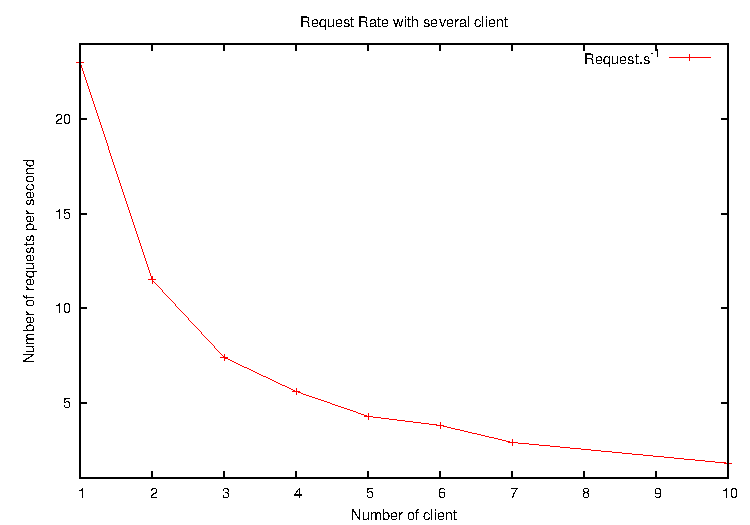
\includegraphics{concurency}
    \caption{Requests per second depending the number of clients}
    \label{fig:Concurrency}
  \end{center}
\end{figure}



In this graphic, we displayed the mean of requests rate from the client side. 
Observing this graphic, we can assume that, right now, Rudy is not able to handle properly several concurrent connexions. 

\section{Conclusions}
 
First, we learned a little about how to build a simple parser in a functional language like Erlang. Something which is actually not obvious.
In addition, in this preliminary work, we discovered that one of the main issues of distributed systems is the handling of concurrency. which give us something to start with in the next seminar.



\end{document}
